%----------------------------------------------------------------%
%--------------------------GRUNDEINSTELLUNGEN--------------------%
%----------------------------------------------------------------%
\documentclass[oneside, ngerman, footinclude=off, captions=tableheading]{scrartcl}
%	'oneside'/'twoside': nicht zwischen linker und rechter Seite unterscheiden (alternativ twoside)
%	'twocolumn': wuerde 2 Spalten auf dem Blatt platzieren
%	'bibliography=totocnumbered': Normal nummeriertes Inhaltsverzeichnis (Kapitelnummer)
%	'listof=totocnumbered': Abbildungs- und Tabellenverzeichnis normal nummeriert (Kapitelnummer)
%	'ngerman' verwendet deutsch als Dokumentensprache (z.B. fuer Sirange)
%	'footinclude=off': Zaehlt Fusszeile zum Rand (vergroessert den Textbereich)
%	'captions=tableheading': Tabellenueberschriften explizit verwenden, erhoeht den Abstand zur Tabelle

\usepackage[ngerman]{babel}		%	Einstellen der Sprache
\usepackage[T1]{fontenc}		%	Wie wird Text ausgegeben, d.h. im PDF
\usepackage[utf8]{inputenc}		%	Welche Zeichen 'versteht' LaTeX bei der Eingabe?
\usepackage{lmodern}			%	Laedt Schriften, die geglaettet sind
\usepackage{blindtext}			%	Beispieltext, zum Testen geeignet

%----------------------------------------------------------------%
%--------------------------ABSTÄNDE------------------------------%
%----------------------------------------------------------------%
%\usepackage[onehalfspacing]{setspace}				%	Für Zeilenabstaende: 'singlespacing' (einfach), 'onehalfspacing' (1.5-fach), 'doublespacing' (2fach)
%\setlength{\parindent}{0cm}						%	Laengenangabe für die Einrueckung der ersten Zeile eines neuen Absatzes.
%\setlength{\parskip}{6pt plus 3pt minus 3pt}		%	Laengenangabe für den Abstand zwischen zwei Absaetzen.
%	Wenn diese beiden Befehle nicht kommentiert sind, wird ein Absatz nicht eingezogen sondern es gibt einen Abstand

% kleinere Abstände über und unter Gleichungen
\usepackage{setspace}\onehalfspacing
\AtBeginDocument{%
  \addtolength\abovedisplayskip{-0.2\baselineskip}
  \addtolength\belowdisplayskip{-0.2\baselineskip}
}

%----------------------------------------------------------------%
%--------------------------MATHE---------------------------------%
%----------------------------------------------------------------%
\usepackage[]{mathtools}							%	Erweiterung von AMSMath, laedt automatisch AMSMath - für viele Mathe-Werkzeuge, 'fleqn' als Option ist für Mathe linksbuendig
\usepackage{amsfonts}								%	Für eine Vielzahl an mathematischen Symbolen
\usepackage{nicefrac}

%----------------------------------------------------------------%
%--------------------------KOPF- UND FUSSZEILEN------------------%
%----------------------------------------------------------------%
\usepackage[automark,headsepline=.4pt]{scrlayer-scrpage}
\pagestyle{scrheadings}
\setkomafont{pageheadfoot}{\normalfont\bfseries}	%	Normale Schriftart und Fett für den Seitenkopf
\addtokomafont{pagenumber}{\normalfont\bfseries}	%	Normale Schriftart und Fett für die Seitenzahl
\clearpairofpagestyles								%	Löscht die Seitenkopf- und Seitenzahlen
\ohead{\thepage}									%	Rechter Seitenkopf mit Seitenzahl
\ihead{\headmark}									%	Linker Seitenkopf mit section
\ofoot[]{\empty}									%	Leere Fußzeile, ungerade Seiten
%	Definert man oben in der documentclass 'twoside', so wird zwischen geraden und ungeraden Seiten unterschieden (NUR DANN!)

%----------------------------------------------------------------%
%--------------------------BILDER--------------------------------%
%----------------------------------------------------------------%
\usepackage{graphicx}									%	Um Bilder einbinden zu koennen 
\usepackage[dvipsnames,svgnames,table]{xcolor}			%	Farben verwenden, Versch. Farbdefinitionen, Farben in Tabellen (-Reihen, -Spalten)
\usepackage{pdfpages}									%	pdfs importieren
\definecolor{Seeblau100}{RGB}{0,169,224}				%	Uni-Farben, z.B. fuer Tabellen
\definecolor{Seeblau65}{RGB}{89,199,254}
\definecolor{Seeblau35}{RGB}{165,224,254}
\definecolor{Seeblau20}{RGB}{203,237,254}
\definecolor{Seegrau60}{RGB}{102,102,102}
\definecolor{Seegrau40}{RGB}{153,153,153}
\definecolor{Seegrau20}{RGB}{204,204,204}
\definecolor{Seegrau10}{RGB}{230,230,230}

%----------------------------------------------------------------%
%--------------------------POSITIONIERUNG------------------------%
%----------------------------------------------------------------%
\usepackage{float}

%----------------------------------------------------------------%
%--------------------------LISTEN--------------------------------%
%----------------------------------------------------------------%
\usepackage{enumitem}							%	Um Listen / Aufzaehlungen leichter zu modifizieren
%\setlist{noitemsep}							%	Verringert den Abstand in Aufzaehlungen

%----------------------------------------------------------------%
%--------TABELLEN-/BILDUNTERSCHRIFTEN und NUMMERIERUNG-----------%
%----------------------------------------------------------------%
\addtokomafont{captionlabel}{\bfseries}			%	Abbildung X.Y wir fett geschrieben
\setcapindent{2em}								%	2. Zeile teilweise haengend und eingezogen. Wenn ganz haengend gewuenscht, auskommentieren


%----------------------------------------------------------------%
%--------------------------LITERATURVERZEICHNIS------------------%
%----------------------------------------------------------------%
\usepackage[german]{babelbib}					%	Bereitstellung des deutschen Layouts fuer die Bibliography
\bibliographystyle{babalpha}

%----------------------------------------------------------------%
%--------------------------SIUNITX-------------------------------%
%----------------------------------------------------------------%
\usepackage[]{siunitx}
\DeclareSIUnit\octave{oct}
\DeclareSIUnit\Hz{Hz}
\sisetup{locale = DE}							%	Automatische Einstellung der Ausgabe für bestimmte Regionen (UK, US, DE, FR, ZA)
\sisetup{separate-uncertainty = false
}

%----------------------------------------------------------------%
%--------------------------URLs / REFs---------------------------%
%----------------------------------------------------------------%
\usepackage[hidelinks]{hyperref}				%	Erweiterte Referenzierung ('hidelinks' verhindert Linien um Links)

%----------------------------------------------------------------%
%--------------------------EIGENE BEFEHLE------------------------%
%----------------------------------------------------------------%

\usepackage{todonotes}
\usepackage{wrapfig}
\setlength{\intextsep}{0pt}%
\usepackage{multicol}

\usepackage{listings}
\usepackage{xcolor}

\definecolor{codegreen}{rgb}{0,0.6,0}
\definecolor{codegray}{rgb}{0.5,0.5,0.5}
\definecolor{codepurple}{rgb}{0.58,0,0.82}
\definecolor{backcolour}{rgb}{0.95,0.95,0.92}

\lstdefinestyle{mystyle}{  
    commentstyle=\color{codegreen},
    keywordstyle=\color{magenta},
    numberstyle=\tiny\color{codegray},
    stringstyle=\color{codepurple},
    basicstyle=\ttfamily\footnotesize,
    breakatwhitespace=false,         
    breaklines=true,                 
    captionpos=t,                    
    keepspaces=true,                 
    numbers=left,                    
    numbersep=5pt,                  
    showspaces=false,                
    showstringspaces=false,
    showtabs=false,                  
    tabsize=2
}


\lstset{style=mystyle}


\begin{document}

\title{Computerphysik I: Blatt 03}
\author{Aurel Müller-Schönau und Leon Oleschko}
\maketitle

\begin{figure*}[h!]
	\centering
	\includegraphics[width=\linewidth]{A_plot.pdf}
	\caption{Fehler in Abhängigkeit von der Schrittweite $H$}
	\label{fig:fehler}
\end{figure*}


\section*{a) Fehlerabhängigkeit}
Um die Fehlerabhängigkeit von verschiedenen numerischen Methoden zu prüfen, wurde ein harmonischer Oszillator (Periodendauer $T$) für $500$ Oszillationen mit verschiedenen Zeitlichen Auflösungen $H$ simuliert. Dabei ist $H\in[0.001;0.001;0.5]/2\pi T$. 
Dies ist zwar unrealistisch hoch, lässt dafür aber eine schnelle Simulation zu.

In der Abbildung \ref{fig:fehler} sind der relative Auslenkungsfehler $x$, der Geschwindigkeitsfehler $v$ und Energiefehler $E$ für verschiedene Zeitauflösungen $H$ dargestellt.

Dass die Energie nur beim Leap-Frog- und Verlet-Verfahren erhalten ist (zumindest beinahe) ist trotzdem gut zu erkennen.
Diese beiden liefern auch nahezu dieselben Ergebnisse, was nicht verwunderlich ist, da beide symmetrische Zweischrittverfahren sind. Die Energie ist erhalten, weil die Schwingung des harmonischen Oszillators unter Zeitumkehr invariant ist, somit ist die Symmetrie der Verfahren hinreichend für Energieerhaltung.

Für kleine Schrittweiten ist das Runge-Kutta-Verfahren beinahe genau so gut wie die symmetrischen Verfahren. Für komplexere Systeme sollte es sogar bessere Ergebnisse liefern aufgrund höherer Konsistenzordnung, jedoch haben die symmetrischen Verfahren in diesem Fall einen systematischen Vorteil.

Das explizite Euler-Cauchy-Verfahren schneidet als nicht symmetrisches Einschrittverfahren am schlechtesten ab. Der "Energiegewinn" ist dadurch zu erklären, dass das Verfahren prinzipbedingt in den Bereichen, in denen die exakte Lösung eine Krümmung besitzt quasi zu weit ausschwenkt, deshalb wird die Schwingungsamplitude immer größer und die Energie wächst immer weiter an.


\section*{b) Phasendiagram}
\begin{figure}[h!]
	\centering
	\includegraphics[width=400pt]{B_Phase.pdf}
	\caption{Phasendiagram für verschiedene Dämpfungen $\gamma$}
	\label{fig:phase}
\end{figure}
In Abbildung \ref{fig:phase} ist das Phasendiagramm für verschiedene Dämpfungen $\gamma$ dargestellt.\\
Die Ortskoordinate $x$ ist mit dem Verlet Verfahren simuliert und die Geschwindigkeit $v$ wird mir der numerischen rechts Ableitung bestimmt.

\section*{c,d,e) Angetriebener Oszillator}
\begin{figure}[t]
	\centering
	\includegraphics[width=290pt]{C_Seite.pdf}
	\caption{Resonanzkurve für 6 verschiedene Dämpfungen $\gamma$}
	\label{fig:seite}
\end{figure}

\paragraph*{c)} In der Abbildung \ref{fig:seite} ist die Resonanzkurve eines harmonischen Oszillators mit Eingenfrequenz $\omega_E$, mit einer Antreibenden Frequenz $\omega_t$ und einer Amplitude der Antreibenden Kraft von $1$ für 6 verschiedene Dämpfungen $\gamma$  dargestellt.\\ 
Dabei wird der Ort mit dem Verlet Verfahren simuliert und die Geschwindigkeit wird mit der numerischen rechts Ableitung bestimmt.
Nach einer Einschwingzeit von $\SI{180}{\radian}\;\omega_E^{-1}$ wird die Amplitude bestimmt, indem das Maximum gespeichert wird, bis nach weitere $\SI{120}{\radian}\;\omega_E^{-1}$ das Maximum ausgelesen wird. 

\smallskip

\begin{figure}[p]
	\centering
	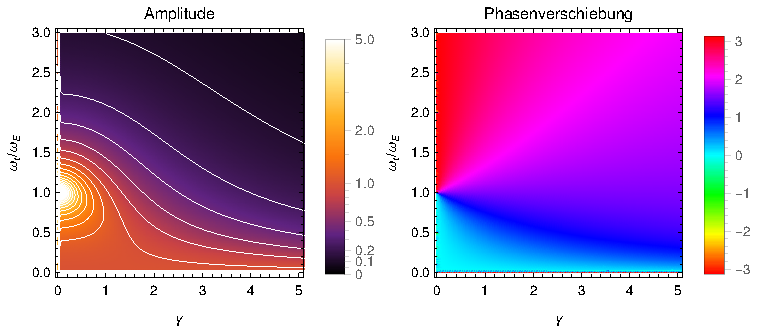
\includegraphics[width=450pt]{C_Plot.pdf}
	\caption{2D Resonanzkurve für verschiedene Dämpfungen $\gamma$ mit Phasenverschiebung zur antreibenden Schwingung in \si{\radian}.}
	\label{fig:plot}
\end{figure}
\paragraph*{e)} Indem an dem Maximumszeitpunkt die Phase der antreibenden Schwingung $\omega_T \cdot t \mod 2\pi$ gespeichert wird, kann auch die Phasenverschiebung zwischen der antreibenden und resultierenden Schwingung bestimmt werden.
Diese ist in $rad$ in der Abbildung \ref{fig:plot} dargestellt.
Dabei ist schön der Phasensprung von $\pi$ bei der Resonanzkatastrophe bei schwacher Dämpfung zu sehen.

\begin{figure}[p]
	\centering
	\includegraphics[width=400pt]{C_3D.pdf}
	\caption{3D Darstellung der Resonanzkurve für verschiedene Dämpfungen $\gamma$}
	\label{fig:3d}
\end{figure}
\paragraph*{d)}
In Abbildung \ref{fig:3d} ist das Phasendiagramme für verschiedene Dämpfungen $\gamma$ als 3 dimensionale Oberfläche dargestellt.

\end{document}